% --- Insertar en Threats to Validity, junto al punto sobre estudios preprint ---
% Sustituye o complementa la oración existente:
% "First, the dataset includes a proportion of preprint studies that may not
%  have undergone full peer review, which could affect the reliability of
%  some findings. However, these studies were evaluated using a structured
%  quality assessment framework to mitigate this risk."

First, the dataset includes a proportion of preprint studies that may not have undergone full peer review, which could affect the reliability of some findings. As shown in Fig.~\ref{fig:item_type}, preprints account for 38.8\% of the corpus (n=121), followed by conference papers (31.1\%, n=97), journal articles (27.9\%, n=87), theses (1.9\%, n=6), and a single book section (0.3\%, n=1). However, these studies were evaluated using the same structured quality-assessment framework described in Section 2.7, which mitigates this risk by weighting conclusions toward CORE and A1/A2 evidence rather than publication venue alone.

\begin{figure}[h]
    \centering
    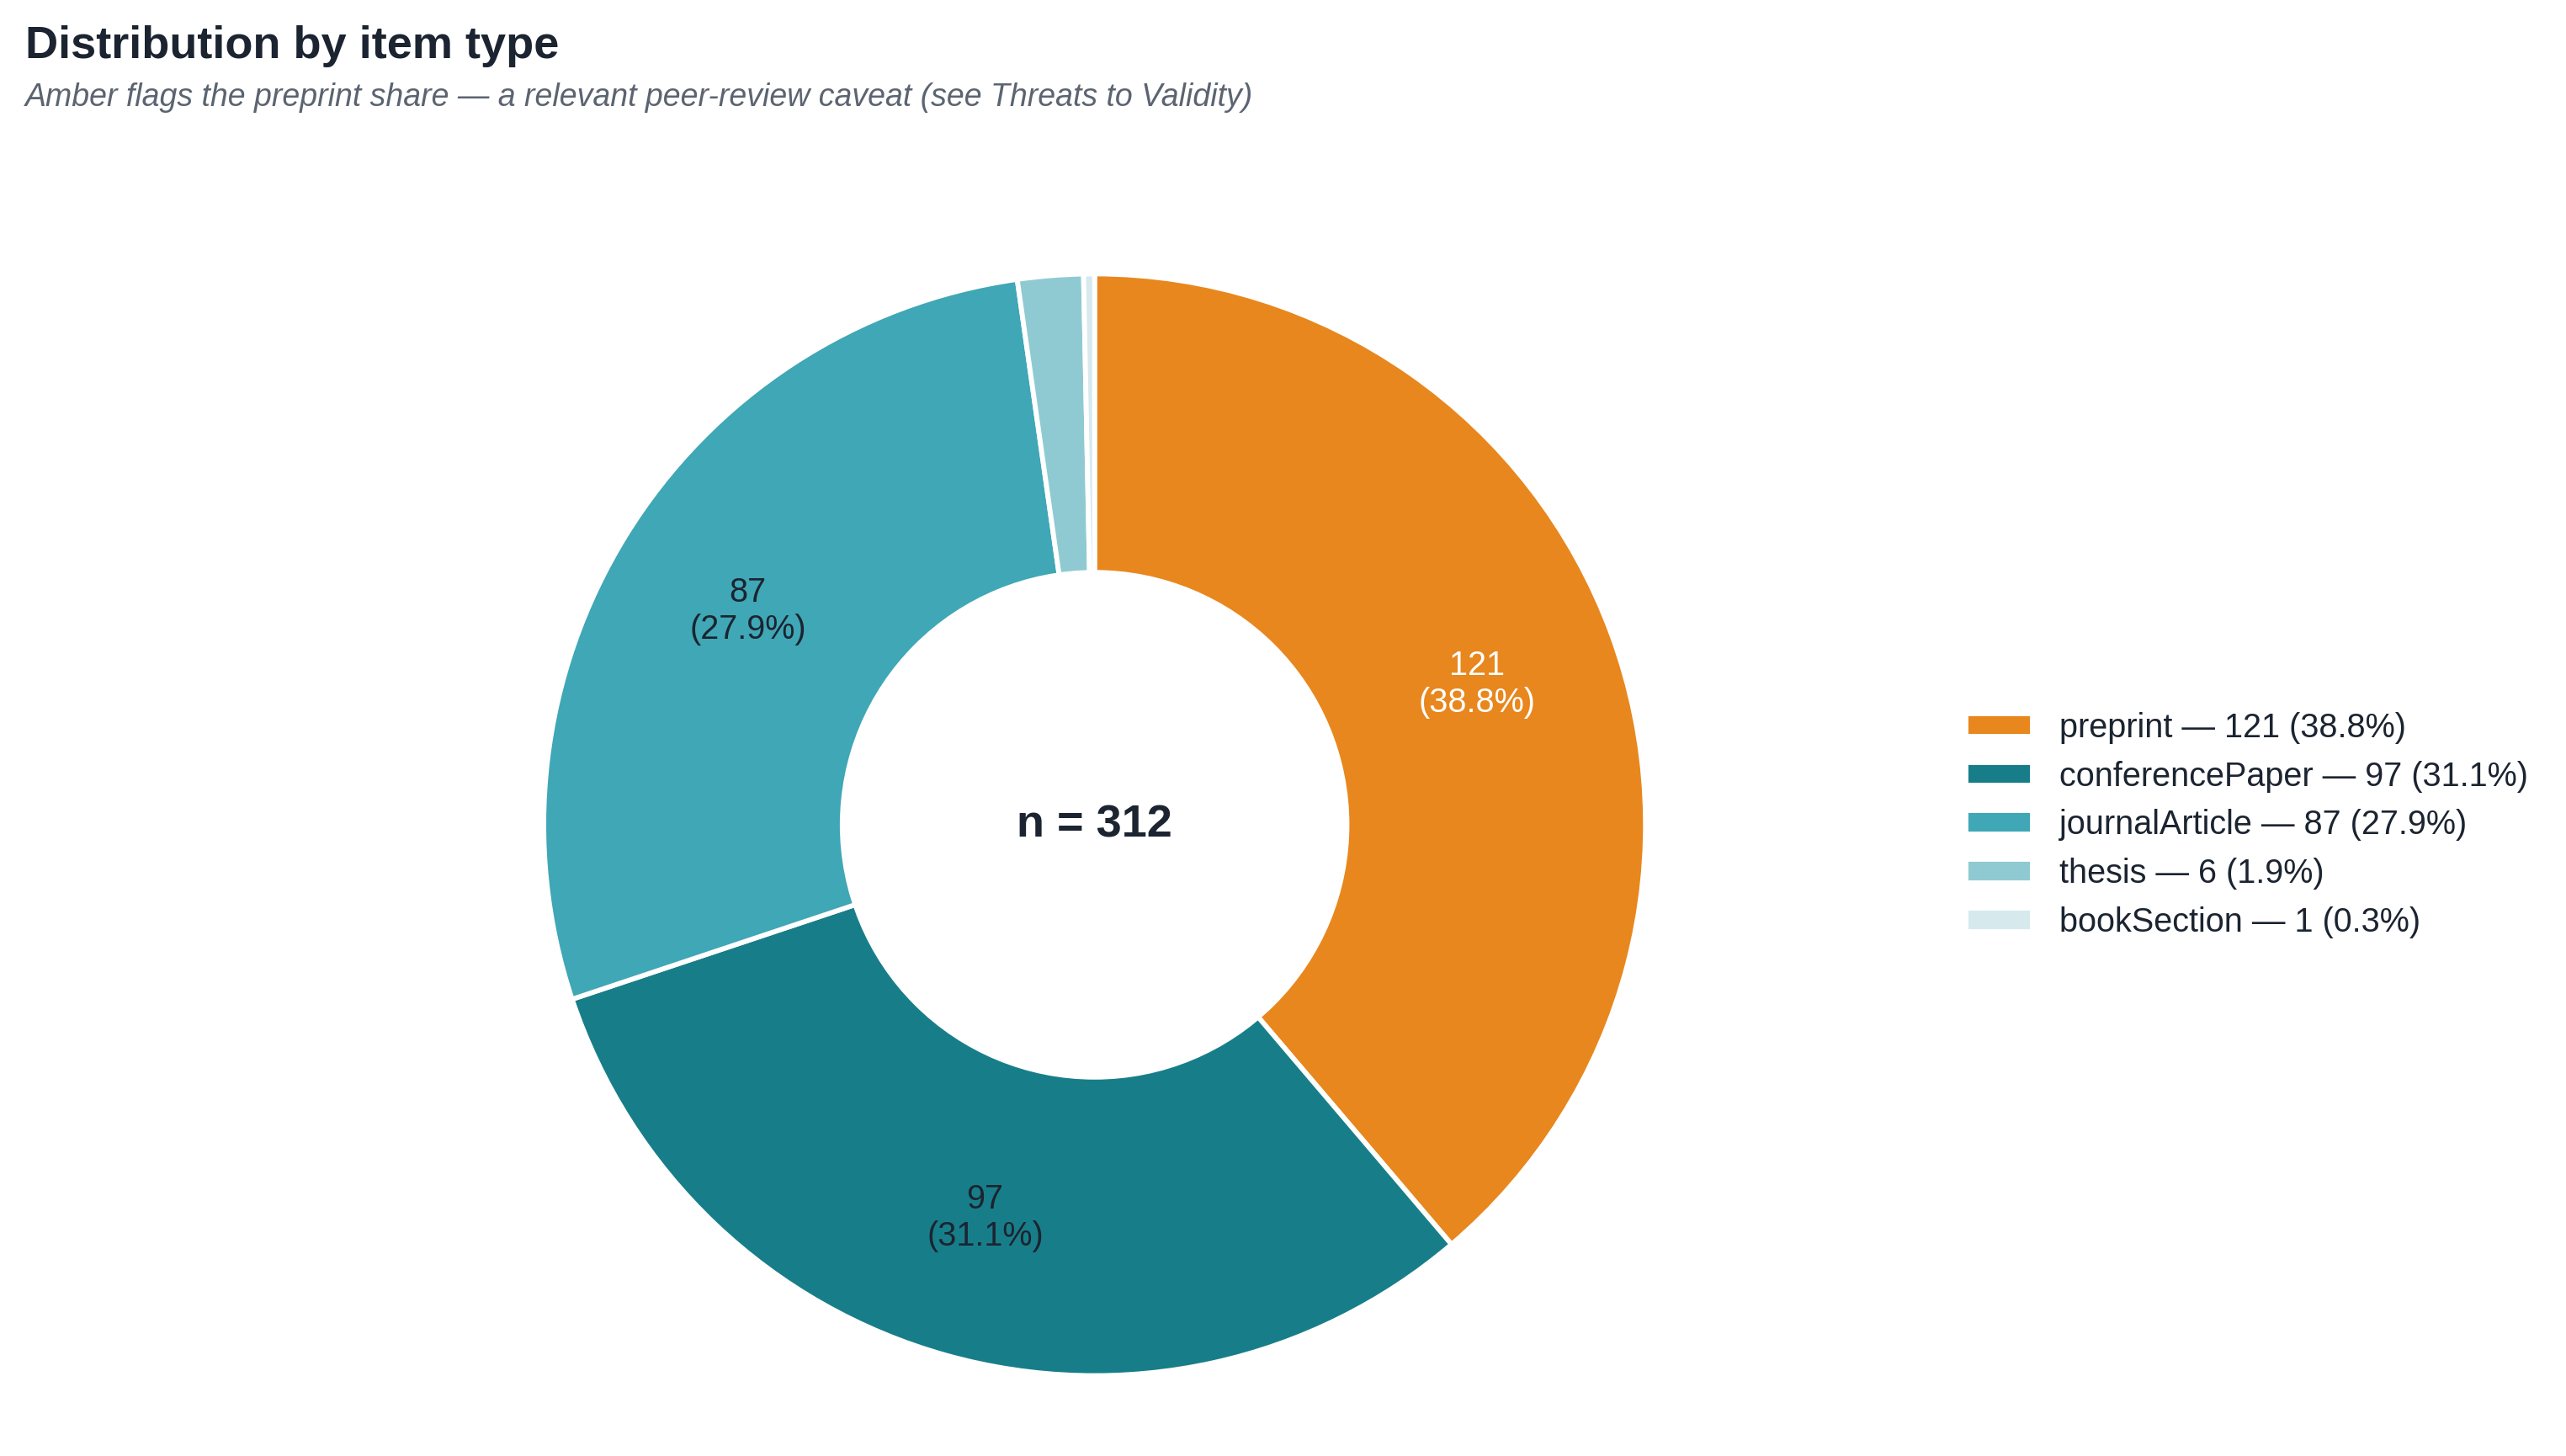
\includegraphics[width=0.82\linewidth]{figures/A3_item_type_distribution.png}
    \caption{Distribution of the corpus by item type. Amber flags the preprint share, the relevant peer-review caveat discussed here.}
    \label{fig:item_type}
\end{figure}
